% Copyright 2004 by Till Tantau <tantau@users.sourceforge.net>.
%
% In principle, this file can be redistributed and/or modified under
% the terms of the GNU Public License, version 2.
%
% However, this file is supposed to be a template to be modified
% for your own needs. For this reason, if you use this file as a
% template and not specifically distribute it as part of a another
% package/program, I grant the extra permission to freely copy and
% modify this file as you see fit and even to delete this copyright
% notice. 

\documentclass{beamer}

% There are many different themes available for Beamer. A comprehensive
% list with examples is given here:
% http://deic.uab.es/~iblanes/beamer_gallery/index_by_theme.html
% You can uncomment the themes below if you would like to use a different
% one:
%\usetheme{AnnArbor}
%\usetheme{Antibes}
%\usetheme{Bergen}
%\usetheme{Berkeley}
%\usetheme{Berlin}
%\usetheme{Boadilla}
%\usetheme{boxes}
%\usetheme{CambridgeUS}
%\usetheme{Copenhagen}
%\usetheme{Darmstadt}
%\usetheme{default}
%\usetheme{Frankfurt}
%\usetheme{Goettingen}
%\usetheme{Hannover}
%\usetheme{Ilmenau}
%\usetheme{JuanLesPins}
%\usetheme{Luebeck}
\usetheme{Madrid}
%\usetheme{Malmoe}
%\usetheme{Marburg}
%\usetheme{Montpellier}
%\usetheme{PaloAlto}
%\usetheme{Pittsburgh}
%\usetheme{Rochester}
%\usetheme{Singapore}
%\usetheme{Szeged}
%\usetheme{Warsaw}


% Customize Warsaw color 
\setbeamercolor*{palette primary}{use=structure,fg=white,bg=red!50!black}
\setbeamercolor*{palette secondary}{use=structure,fg=white,bg=red!60!black}
\setbeamercolor*{palette tertiary}{use=structure,fg=white,bg=red!70!black}

% Customize Warsaw block title and background colors
\setbeamercolor{block title}{bg=red!50!black,fg=white}

\title[Multi-Robot Localization]{Multi-robot Localization}


% % A subtitle is optional and this may be deleted
\subtitle{Application to Area Coverage Optimization}

\author[C.~Lu]{Caleb~Lu  \\\and
Advisor: Dr. Suruz Miah}
% - Give the names in the same order as the appear in the paper.
% - Use the \inst{?} command only if the authors have different
%   affiliation.

\institute[Bradley University] % (optional, but mostly needed)
{
  Department of Electrical and Computer Engineering\\
  Bradley University\\
  1501 W. Bradley Avenue\\
  Peoria, IL, 61625, USA
}
% - Use the \inst command only if there are several affiliations.
% - Keep it simple, no one is interested in your street address.

\date[June~7,~2019]{Friday, June~07,~2019}
% - Either use conference name or its abbreviation.
% - Not really informative to the audience, more for people (including
%   yourself) who are reading the slides online

\logo{\hfill\href{http://www.bradley.edu}{
\includegraphics[width=0.75cm]{figs/logoBU1-Print}}}  % place logo in every page 


\subject{Mobile Robot Localization}
% This is only inserted into the PDF information catalog. Can be left
% out. 

% If you have a file called "university-logo-filename.xxx", where xxx
% is a graphic format that can be processed by latex or pdflatex,
% resp., then you can add a logo as follows:

% \pgfdeclareimage[height=0.5cm]{university-logo}{university-logo-filename}
% \logo{\pgfuseimage{university-logo}}

% Delete this, if you do not want the table of contents to pop up at
% the beginning of each subsection:
%\AtBeginSubsection[]
%{
 % \begin{frame}<beamer>{Outline}
  %  \tableofcontents[currentsection,currentsubsection]
  %\end{frame}
%}

% Let's get started
\begin{document}

\begin{frame}
  \titlepage
\end{frame}

\begin{frame}{Outline}
  \tableofcontents
  \setcounter{tocdepth}{1}
  % You might wish to add the option [pausesections]
\end{frame}

% Section and subsections will appear in the presentation overview
% and table of contents.
\section{Introduction}
\subsection{What is Localization?}
\begin{frame}{Introduction}{What is Localization?}
  
\begin{itemize}
  \item
   For robot navigation, it is important to have a means of determining the location of the robot. Localization allows for accurate determination of a robots position in an In-Door or Out-Door environment.
   \item
    The main focus of this project is using In-Door Localization to determine the position of the robot. This will be accomplished by using the position of three beacons with known positions to the robot and the line of sight distance from each beacon to the robot.
  \end{itemize}
  \begin{figure}
  
\includegraphics[scale=0.2]{figs/img/Lu_Images/locationIcon}
  \caption{Location Markers}
  \end{figure}
  
\end{frame}

%----------------------------------
\subsection{How In-Door Localization is Executed}
\begin{frame}{Introduction}{In-Door Localization}
\begin{itemize}
\item
 The goal for In-Door Localization, in this case, is to use Radio Frequency IDentification (RFID) system to determine the Radio Signal Strength (RSS). By using the RSS and the RFID system, the line of sight distance can be determined. 
 \item
 By using the method of trilateration, the known position of the beacons, and the line of sight distance; the position of the robot can be determined.
\end{itemize}
\begin{figure}
\centering

\includegraphics[scale=0.2]{figs/img/Lu_Images/indoorIcon}
\end{figure}
\end{frame}
%----------------------------------


\section{Sensors}

\subsection{Interoceptive Sensors}

\begin{frame}{Sensor Types}{Interoceptive Sensors}
Interoceptive Sensors are sensors that pertain to the robot's on-board functional components. Example of Interoceptive Sensors would be:

\begin{itemize}
\item Wheel Encoders
\item Heading Angle
\item Battery Status
\end{itemize}

\begin{figure}
\centering
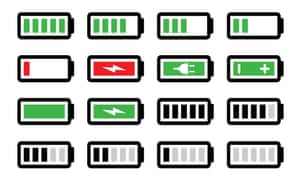
\includegraphics[scale=0.5]{figs/img/Lu_Images/batteryStatus}
\end{figure}
  
\end{frame}
%----------------------------------

\subsection{Exteroceptive Sensors}

\begin{frame}{Sensor Types}{Exteroceptive Sensors}
Exteroceptive Sensors are sensors that read data from the robot's work space/environment. Examples of Exteroceptive Sensors would be:
\begin{itemize}
\item Range measurement to object
\item Light intensity
\item Images captured by camera
\item Microphone Data
\end{itemize}
\begin{figure}
\centering
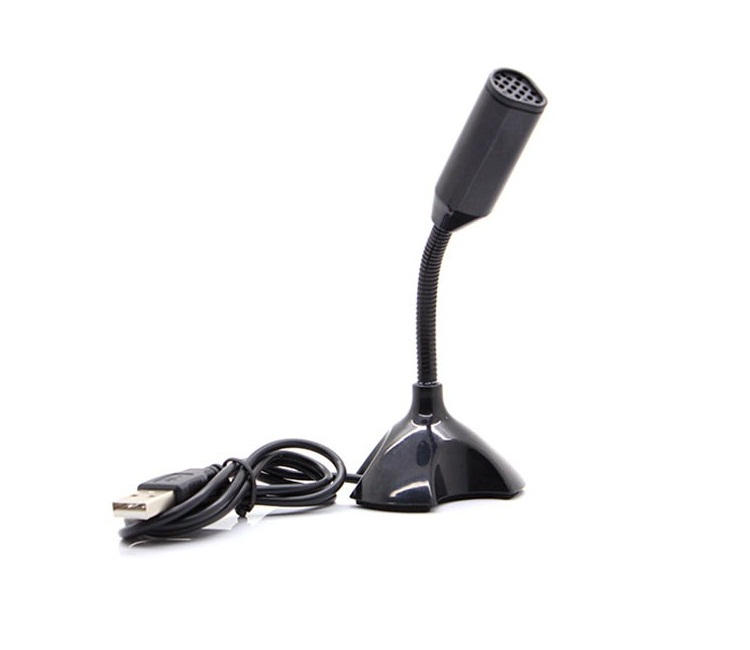
\includegraphics[scale=0.4]{figs/img/Lu_Images/microphone}
\end{figure}
  
\end{frame}

%----------------------------------
\subsection{Sensors in Localization}
\begin{frame}{Sensors in Localization}
\begin{itemize}
\item
Mainly exteroceptive sensors will be used for localization. RSS will be used to determine line of sight distance.
\item
Interoceptive sensors will be used to help determine where the robot moves based on the position determined from localization.
\end{itemize}


\end{frame}

%----------------------------------

\section{Other Popular Localization Techniques}
	
\begin{frame}{Other Localization Techniques}

\begin{itemize}
\item External Kalmen Filter (EFK)

\item Unscented Kalmen Filter (UFK)

\end{itemize}

\end{frame}
%----------------------------------


\section{Caley-Meger Determinant}


\begin{frame}{Localization through Trilateration}
Trilateration is the method of determining position by using the known positions of three beacons and the line of sight distance to each beacon.

\begin{figure}
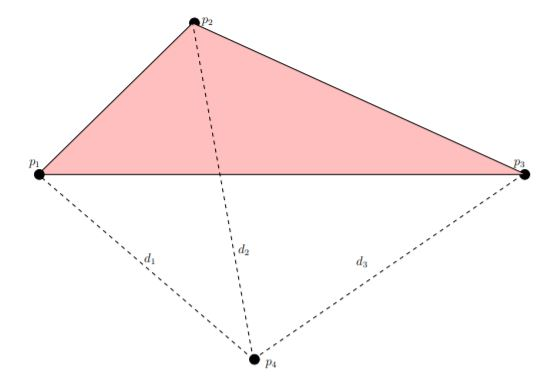
\includegraphics[scale=0.7]{figs/img/Lu_images/robotTrilaterationDiagram}
\caption{Trilateration Diagram}
\end{figure}  

\end{frame}

%----------------------------------
\begin{frame}{What is the Caley-Meger Determinant?}
For trilateration, the equation found for the robot is:

\begin{figure}
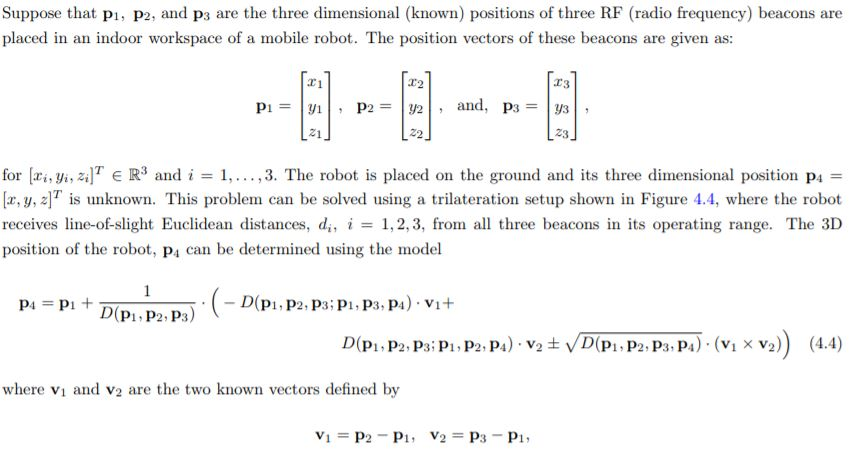
\includegraphics[scale=0.6]{figs/img/Lu_Images/caleyMegerEquations1}
\end{figure}  

\end{frame}

%----------------------------------
\begin{frame}{What is the Caley-Meger Determinant?}
\begin{figure}
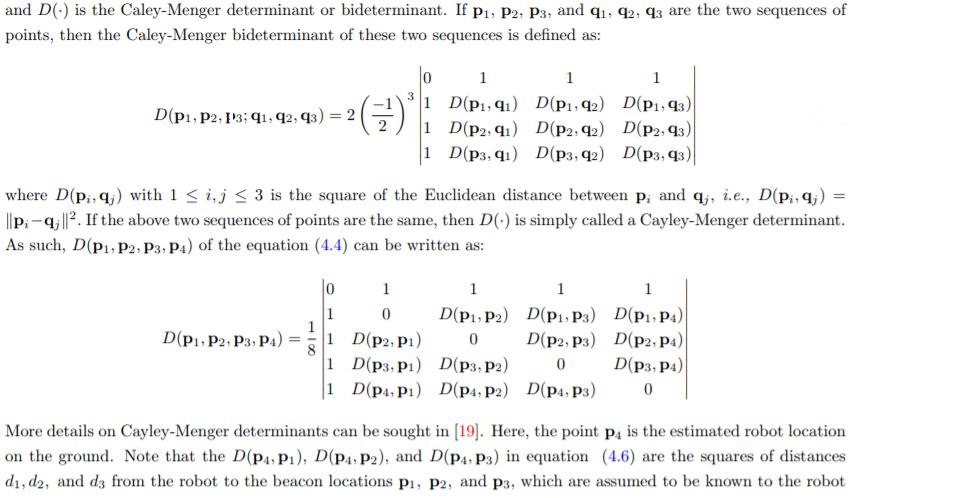
\includegraphics[scale=0.6]{figs/img/Lu_Images/caleyMegerEquations2}
\end{figure}  

\end{frame}

%----------------------------------
\begin{frame}{What is the Caley-Meger Determinant?}
\begin{figure}
\centering
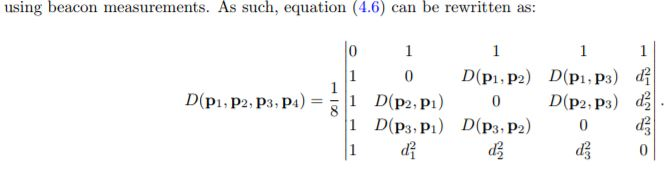
\includegraphics[scale=0.8]{figs/img/Lu_Images/caleyMegerEquations3}
\end{figure}  

\end{frame}

%----------------------------------



\section{Caley-Meger Determinant Example}


\begin{frame}{Caley-Meger Determinant Example}

\begin{figure}
\centering
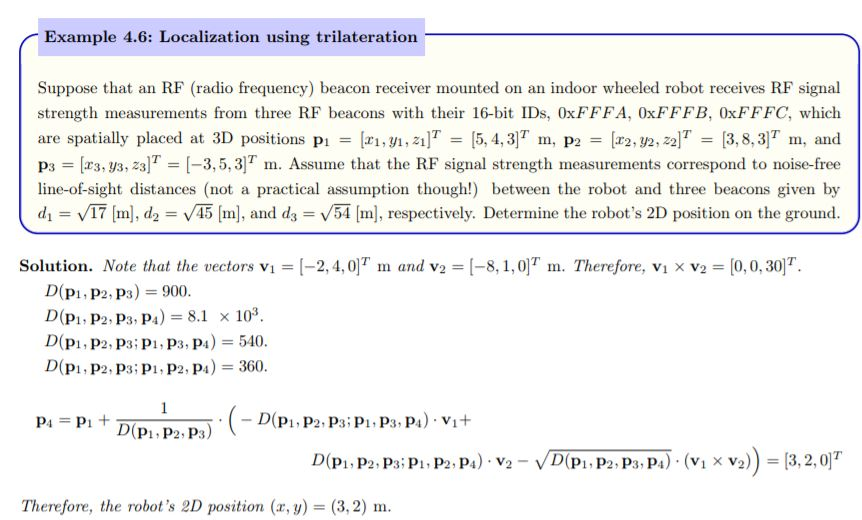
\includegraphics[scale=0.6]{figs/img/Lu_images/cmExample}
\end{figure}  

\end{frame}

%----------------------------------

\section{Future Plans - Incoming Week}


\begin{frame}{Future Plans - Incoming Week}

\begin{itemize}
\item To be determined
\end{itemize}


\end{frame}

%----------------------------------



% You can reveal the parts of a slide one at a time
% with the \pause command:
%\begin{frame}{Second Slide Title}
%  \begin{itemize}
%  \item {
%    First item.
%    \pause % The slide will pause after showing the first item
%  }
  %\item {   
  %  Second item.
 % }
  % You can also specify when the content should appear
  % by using <n->:
 % \item<3-> {
 %   Third item.
 % }
%  \item<4-> {
%    Fourth item.
 % }
  % or you can use the \uncover command to reveal general
  % content (not just \items):
%  \item<5-> {
%    Fifth item. \uncover<6->{Extra text in the fifth item.}
%  }
%  \end{itemize}
%\end{frame}

%\section{Second Main Section}

%\subsection{Another Subsection}

%\begin{frame}{Blocks}
%\begin{block}{Block Title}
%You can also highlight sections of your %presentation in a block, with it's own %title
%\end{block}
%\begin{theorem}
%There are separate environments for %theorems, examples, definitions and proofs.
%\end{theorem}
%\begin{example}
%Here is an example of an example block.
%\end{example}
%\end{frame}

% Placing a * after \section means it will not show in the
% outline or table of contents.
\section*{Questions}
\begin{frame}{}
  \centering \Huge
  \emph{Questions?}
\end{frame}


\end{document}



%%% Local Variables:
%%% mode: latex
%%% TeX-master: t
%%% End:
\grid
<<<<<<< HEAD
=======
=======
% Copyright 2004 by Till Tantau <tantau@users.sourceforge.net>.
%
% In principle, this file can be redistributed and/or modified under
% the terms of the GNU Public License, version 2.
%
% However, this file is supposed to be a template to be modified
% for your own needs. For this reason, if you use this file as a
% template and not specifically distribute it as part of a another
% package/program, I grant the extra permission to freely copy and
% modify this file as you see fit and even to delete this copyright
% notice. 

\documentclass{beamer}

% There are many different themes available for Beamer. A comprehensive
% list with examples is given here:
% http://deic.uab.es/~iblanes/beamer_gallery/index_by_theme.html
% You can uncomment the themes below if you would like to use a different
% one:
%\usetheme{AnnArbor}
%\usetheme{Antibes}
%\usetheme{Bergen}
%\usetheme{Berkeley}
%\usetheme{Berlin}
%\usetheme{Boadilla}
%\usetheme{boxes}
%\usetheme{CambridgeUS}
%\usetheme{Copenhagen}
%\usetheme{Darmstadt}
%\usetheme{default}
%\usetheme{Frankfurt}
%\usetheme{Goettingen}
%\usetheme{Hannover}
%\usetheme{Ilmenau}
%\usetheme{JuanLesPins}
%\usetheme{Luebeck}
\usetheme{Madrid}
%\usetheme{Malmoe}
%\usetheme{Marburg}
%\usetheme{Montpellier}
%\usetheme{PaloAlto}
%\usetheme{Pittsburgh}
%\usetheme{Rochester}
%\usetheme{Singapore}
%\usetheme{Szeged}
%\usetheme{Warsaw}


% Customize Warsaw color 
\setbeamercolor*{palette primary}{use=structure,fg=white,bg=red!50!black}
\setbeamercolor*{palette secondary}{use=structure,fg=white,bg=red!60!black}
\setbeamercolor*{palette tertiary}{use=structure,fg=white,bg=red!70!black}

% Customize Warsaw block title and background colors
\setbeamercolor{block title}{bg=red!50!black,fg=white}

\title[Intro to ROS]{Introduction to Robot Operating System (ROS)}

% % A subtitle is optional and this may be deleted
% \subtitle{Product Proposal}

\author[A.Elhussein]{Amr~Elhussein  \\\and
Advisor: Dr. Suruz Miah}
% - Give the names in the same order as the appear in the paper.
% - Use the \inst{?} command only if the authors have different
%   affiliation.

\institute[Bradley University] % (optional, but mostly needed)
{
  Department of Electrical and Computer Engineering\\
  Bradley University\\
  1501 W. Bradley Avenue\\
  Peoria, IL, 61625, USA
}
% - Use the \inst command only if there are several affiliations.
% - Keep it simple, no one is interested in your street address.

\date[May~31,~2019]{Friday, May~31,~2019}
% - Either use conference name or its abbreviation.
% - Not really informative to the audience, more for people (including
%   yourself) who are reading the slides online


\setbeamertemplate{bibliography item}{\insertbiblabel}  % insert bibliography numbers instead of symbol
\setbeamertemplate{caption}[numbered] % adds the figure or table number to the caption.

\logo{\hfill\href{http://www.bradley.edu}{
\includegraphics[width=0.75cm]{figs/logoBU1-Print}}}  % place logo in every page 


\subject{Mobile Robot Localization}
% This is only inserted into the PDF information catalog. Can be left
% out. 

% If you have a file called "university-logo-filename.xxx", where xxx
% is a graphic format that can be processed by latex or pdflatex,
% resp., then you can add a logo as follows:

% \pgfdeclareimage[height=0.5cm]{university-logo}{university-logo-filename}
% \logo{\pgfuseimage{university-logo}}

% Delete this, if you do not want the table of contents to pop up at
% the beginning of each subsection:
%\AtBeginSubsection[]
%{
 % \begin{frame}<beamer>{Outline}
  %  \tableofcontents[currentsection,currentsubsection]
  %\end{frame}
%}

% Let's get started
\begin{document}

\begin{frame}
  \titlepage
\end{frame}

\begin{frame}{Outline}
  \tableofcontents
  % You might wish to add the option [pausesections]
\end{frame}

% Section and subsections will appear in the presentation overview
% and table of contents.
\section{Introduction}
\subsection{Historical Background}
\begin{frame}{Intrduction}{History and Legacy}
  
\begin{itemize}
  \item
   Started in 2007 by researches from Stanford AI Robot (Stair) and the Personal Robots (PR) Program and was sponsored by Willow Garage a visionary robotics incubator.
  \item
Used Worlwide in Research and Industry.
  \item
    Currently supported by the Open Source Robotics Foundation.
  \end{itemize}
  \begin{figure}
  
  % \includegraphics[scale=0.2]{figs/stair_small}
  \caption{Stair}
  \end{figure}
  
\end{frame}
\subsection{Robot Programming Before ROS}
\begin{frame}{Intrduction}{Robot Programming Before ROS}
\begin{itemize}
  \item
There was no common platform for develeoping robotics and it took ages !
  \item
The developed software for a robot couldn't be used in any other robot.
  \item
  Developers had to implement algorithms on their own.
  \end{itemize}
  
\end{frame}
\subsection{ROS is ..}
\begin{frame}{Intrduction}{ROS is ..}
A flexible framework for writing robot software. It is a collection of tools, libraries, and conventions that aim to simplify the task of creating complex and robust robot behavior across a wide variety of robotic platforms.
  
\end{frame}
\subsection{ROS Equation}
\begin{frame}{Intrduction}{Ros Equation}
\begin{figure}
\centering

% \includegraphics[scale=1.4]{figs/ros_equation}
\end{figure}

  
\end{frame}
%----------------------------------

\section{ROS Concepts}

\subsection{Filesystem}

\begin{frame}{ROS Concepts}{Filesystem}
\begin{figure}
\centering
% \includegraphics[scale=0.4]{figs/filesystem}
\end{figure}
  
\end{frame}

%----------------------------------

\subsection{Computation Graph}

\begin{frame}{ROS Concepts}{Computation Graph}
\begin{figure}
\centering
% \includegraphics[scale=2]{figs/computaiongraph}
\end{figure}
  
\end{frame}
%----------------------------------
\begin{frame}{ROS Concepts}{Computation Graph: Master}
\begin{figure}
\centering
% \includegraphics[scale=0.35]{figs/master}
\end{figure}

\end{frame}
%----------------------------------
\begin{frame}{ROS Concepts}{Computation Graph: Master}
\begin{figure}
\centering
% \includegraphics[scale=0.3]{figs/nodeseg}
\end{figure}
\end{frame}
%----------------------------------


\subsection{Community level}

\begin{frame}{ROS Concepts}{Community level}
\begin{figure}
\centering
% \includegraphics[scale=0.5]{figs/community}
\end{figure}
  
\end{frame}

%----------------------------------

\section{ROS installation}

% put a slide with three dimensional system architecture drawing using ipe
% another slide with explanation

% put a slide with system block diagram

%\subsection{Block Diagram}

\begin{frame}{Installation}

\begin{itemize}
\item Supported for debian-based distributions such as Ubuntu.
\item Supported by many robots.
\item Current supported distributions
\begin{itemize}
\item ROS Kinetic Kame, Released May, 2016.
\item ROS Melodic Morenia, Released May, 2018
%put pics%
\end{itemize}
\end{itemize}

\end{frame}
%----------------------------------
\begin{frame}{Installation}

After choosing the distribution follow the instruction on ROS wiki which start by:
\begin{itemize}
\item Configure your Ubuntu repositories.
\item Setup your sources.list.
\item Set keys
\item Install with "sudo apt-get install ros-kinetic-desktop-full"
\end{itemize}

\end{frame}

%----------------------------------

\section{Future of ROS}


\begin{frame}{Future of ROS}
  
\end{frame}

%----------------------------------



% You can reveal the parts of a slide one at a time
% with the \pause command:
%\begin{frame}{Second Slide Title}
%  \begin{itemize}
%  \item {
%    First item.
%    \pause % The slide will pause after showing the first item
%  }
  %\item {   
  %  Second item.
 % }
  % You can also specify when the content should appear
  % by using <n->:
 % \item<3-> {
 %   Third item.
 % }
%  \item<4-> {
%    Fourth item.
 % }
  % or you can use the \uncover command to reveal general
  % content (not just \items):
%  \item<5-> {
%    Fifth item. \uncover<6->{Extra text in the fifth item.}
%  }
%  \end{itemize}
%\end{frame}

%\section{Second Main Section}

%\subsection{Another Subsection}

%\begin{frame}{Blocks}
%\begin{block}{Block Title}
%You can also highlight sections of your %presentation in a block, with it's own %title
%\end{block}
%\begin{theorem}
%There are separate environments for %theorems, examples, definitions and proofs.
%\end{theorem}
%\begin{example}
%Here is an example of an example block.
%\end{example}
%\end{frame}

% Placing a * after \section means it will not show in the
% outline or table of contents.
\section*{Summary}

\begin{frame}{Summary}
  \begin{itemize}
  \item
    The \alert{first main message} of your talk in one or two lines.
  \item
    The \alert{second main message} of your talk in one or two lines.
  \item
    Perhaps a \alert{third message}, but not more than that.
  \end{itemize}
  
  \begin{itemize}
  \item
    Outlook
    \begin{itemize}
    \item
      Something you haven't solved.
    \item
      Something else you haven't solved.
    \end{itemize}
  \end{itemize}
\end{frame}



% All of the following is optional and typically not needed. 
\appendix
\section<presentation>*{\appendixname}
\subsection<presentation>*{For Further Reading}

\begin{frame}[allowframebreaks]
  \frametitle<presentation>{For Further Reading}
    
  \begin{thebibliography}{10}
    
  \beamertemplatebookbibitems
  % Start with overview books.

  \bibitem{Author1990}
    A.~Author.
    \newblock {\em Handbook of Everything}.
    \newblock Some Press, 1990.
 
    
  \beamertemplatearticlebibitems
  % Followed by interesting articles. Keep the list short. 

  \bibitem{Someone2000}
    S.~Someone.
    \newblock On this and that.
    \newblock {\em Journal of This and That}, 2(1):50--100,
    2000.
  \end{thebibliography}
\end{frame}

\end{document}



%%% Local Variables:
%%% mode: latex
%%% TeX-master: t
%%% End:

